\subsection[]{ Calcolare la "resistenza di irraggiamento" di un circuito elettrico quadrato di lato L, piccolo rispetto alla lunghezza d'onda $\lambda$ della radiazione monocromatica incidente, se il circuito è puramente resistivo con resistenza R.\\
Calcolare anche la sezione d'urto di assorbimento e la sezione d'urto elastica se l'onda incidente ha campo magnetico perpendicolare al piano del circuito e di modulo massimo $B_0$. }
Nomi a parte il problema è schematizzato in Figura:
\begin{figure}[H]
	\centering
	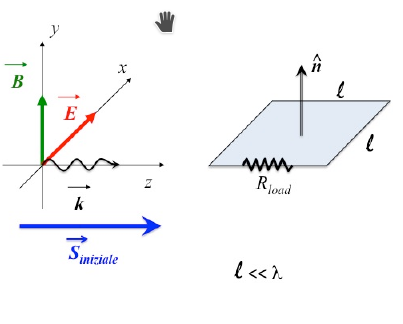
\includegraphics[width=0.5\textwidth]{immagini/spira_onda.png}
	\caption{Spira immersa nel campo di onda e.m.}
	\label{fig:spira1}
\end{figure}
\paragraph{Calcolo della resistenza di irraggiamento.}
I campi ed il vettore di Poynting dell'onda sono:
\[
	\boldsymbol{E} = E_x \hat{i} = E_0 \cos\left( \omega t - kz \right) \hat{i} 
.\] 
\[
	\boldsymbol{B} = B_y \hat{j} = B_0 \cos\left( \omega t - kz \right) \hat{j} 
.\] 
\[
	\boldsymbol{S}_{in} = \frac{E_0^2}{Z_0}\cos\left( \omega t - kz \right) \hat{k} 
.\] 
Sia $I\left( t \right) $ la corrente che scorre nel circuito; possiamo sfruttare le ipotesi di dimensioni piccole (rispetto a $\lambda$) per dire che tale corrente è uniforme in tutta la spira. Trascurando anche autoinduttanza e capacità parassite possiamo affermare che il circuito ha momento di dipolo nullo.\\
Non vale lo stesso per il momento di dipolo magnetico:
\[
	\boldsymbol{p}_m = I\left( t \right) l^2 \hat{j}
.\] 
Adesso aggiungendo le ipotesi di perfetta monocromaticita dell'onda incidente e di nessuna perdita di energia per irraggiamento del circuito si calcola la corrente $I\left( t \right)$ applicando Faraday:   
\[
	\varepsilon\left( t \right) = - \frac{\mbox{d} \Phi\left( \boldsymbol{B} \right) }{\mbox{d} t} = R_{load} I\left( t \right) 
.\]
Mettiamo quindi in mezzo la geometria del circuito:
\[
	I\left( t \right) = \frac{\varepsilon\left( t \right)}{R_{load}} = 
	- \frac{1}{R_{load}} \frac{\mbox{d} \Phi\left( \boldsymbol{B} \right) }{\mbox{d} t} 
	= - \frac{1}{R_{load}} \frac{\mbox{d}}{\mbox{d}t} \left[ \int_{-l/2}^{l/2} B_0 \cos\left( \omega t - kz \right) l dz \right] 
	= \frac{\omega l^2B_0\sin\left( \omega t\right)}{R_{load}} \frac{\sin\left( kl/2 \right)}{kl/2}      
.\] 
Agginungendo l'approssimazione:
\[
	\frac{kl}{2} = \frac{\pi l}{\lambda} \ll 1 \implies I\left( t \right) = \frac{\omega l^2 B_0 \sin\left( \omega t \right) }{R_{load}}  
.\] 
Possiamo allora calcolare la potenza irraggiata:
\[
	P_{el} = \frac{\left| \ddot{\boldsymbol{p_m}} \right| ^2}{6\pi \epsilon_0 c^{5}} = \frac{\ddot{I}^2\left( t \right) l^4}{6\pi \epsilon_0 c^5}
.\] 
Se si effettua un bilancio energetico del circuito:
\[
	\varepsilon I = R_{load}I^2 + P_{el} = R_{load} I^2 + \frac{l^4}{6\pi \epsilon_0 c^5}\ddot{I}^2
.\] 
Nel caso in analisi la f.e.m. è armonica 
\[
	\varepsilon = \varepsilon_0 \sin\left( \omega t \right) \quad 
	\text{ con } \quad  
	\varepsilon_0 = \omega l^2 B_0
\]
Quindi la soluzione stazionaria per la corrente sarà anch'essa armonica: $I = I_0 \sin\left( \omega t \right) $, in conclusione:
\[
	\varepsilon I = R_{load}I^2 + \frac{\omega ^{4}l^{4}}{6\pi \epsilon_0 c^{5}} \implies \varepsilon = \left( R_{load} + R_{irr} \right) I
.\] 
Dove è stata definita la resistenza di irraggiamento (dipendente dalla frequenza):
\[
	R_{irr} = \frac{\omega^4l^4}{6\pi \epsilon_0 c^5}
.\]
Espressa in funzione della lunghezza d'onda:
\[
	R_{irr} = \omega^4 \frac{l^4}{6\pi \epsilon c^5} = \left( \frac{2\pi c}{\lambda} \right) ^4 \frac{l^4\sqrt{\mu_0 \epsilon_0} }{6 \pi \epsilon_0 c^4} = \frac{8}{3}\pi^3 Z_0\left( \frac{l}{\lambda} \right)^4 = 31.1 \text{ k}\Omega \left( \frac{l}{\lambda} \right)^4  
.\] 
\paragraph{Calcolo delle sezioni d'urto.}
Notando che 
\[
	I\left( t \right) = \frac{\varepsilon\left( t \right) }{\left( R_{load} + R_{irr} \right) }
.\] 
Possiamo ottenere la potenza assorbita e la potenza "elastica":
\[
	P_{abs} = R_{load} I^2 = \frac{R_{load}}{\left( R_{load} + R_{irr} \right) ^2}\varepsilon^2
.\] 
\[
P_{el} = R_{irr} I^2 =  \frac{R_{load}}{\left( R_{load} + R_{irr} \right) ^2}\varepsilon^2
.\] 
Quindi la potenza trasferita al carico è massima per $R_{load} = R_{irr}$.\\
Adesso basta mediare il vettore di Poynting per concludere:
\[
\left< \left| \boldsymbol{S}_{in} \right| \right> = \frac{\boldsymbol{E}_0^2}{2Z_0}
.\] 
llora le sezioni d'urto sono:
\[
	\sigma_{abs} = \frac{4\pi^2}{\lambda^2}l^4Z_0 \frac{R_{load}}{\left(R_{load} + R_{irr}\right)^2}
.\] 
\[
	\sigma_{irr} = \frac{4\pi^2}{\lambda^2}l^4Z_0 \frac{R_{irr}}{\left(R_{load} + R_{irr}\right)^2}
.\]
\[
	\sigma_{tot} = \sigma_{irr} + \sigma_{load} = \frac{4\pi^2}{\lambda^2}l^4Z_0 \frac{Z_0}{\left(R_{load} + R_{irr}\right)^2}
.\] 

\subsection[]{ Utilizzando le apposite tabelle che forniscono le masse dei nuclei, determinare il Q-valore o l'energia di soglia dei seguenti processi, valutando l'eventuale ruolo della interazione coulombiana nello stato iniziale:
\begin{enumerate}	
	\item	p + 40Ar $\implies$ p + 39Ar + n 
	\item	p + 14N $\implies$ X + n
	\item	p + 16O $\implies$ X + n
	\item	n + 14N $\implies$ 14C + p
	\item	4He + 14N $\implies$ 17O + p
	\item	2H + 3H $\implies$ 4He + n
	\item	2H + 2H $\implies$ 4He + $\gamma$
	\item	p + 198Hg $\implies$ 197Au + p + p
\end{enumerate}
}
Partiamo con un pò di teoria:
\[
	Q = \sum M_{in} - \sum M_{fin} 
.\] 
Se il Q-valore è positivo allora la reazione avviene in modo spontaneo: l'energia di soglia è nulla.\\
Se il Q-valore è negativo allora l'energia di soglia è maggiore di zero e dipende dalla carica del proiettile.
Se la particella proiettile è neutra allora l'energia di soglia è il modulo del Q-valore, altrimenti è necessario calcolare l'energia necessaria a vincere l'interazione columbiana per arrivare al nucleo (essendo le interazioni sopra scritte tutte forti) nel sistema del laboratorio.\\
Per effettuare il calcolo sfruttiamo la conservazione dell'energia e della quantità di moto non relativistiche in una dimensione, chiariamo la notazione:
\begin{itemize}
	\item $R$: raggio del nucleo colpito 
	\item $m_{prt}$: massa del proiettile.
	\item v$_0$: velocità iniziale del proiettile.
	\item $T$: energia cinetica iniziale del proiettile.
	\item $Z$: protoni del nucleo colpito.
	\item  $M$: massa del nucleo colpito.
	\item $d$: distanza in cui i nuclei si urtano definita dalla somma dei raggi delle due particelle coinvolte:
		 \[
			 d = R + r_{prt} \approx \left( 1.25 A^{1/3} + r_{\text{skin}} + r_{prt} \right) \text{ fm} = \left( 1.25 A^{1/3} + 2 + r_{prt} \right) \text{ fm}  
		.\] 
\end{itemize}
Facendo il conto:
 \[
\begin{cases}
	m_{prt}\text{v}_0 = \left( m_p + M \right)V_{cm}\\
	T \ge \frac{1}{2}\left( m_{prt} + M \right)V_{cm} + \frac{Ze^2}{4\pi \epsilon_0 d} \\
	T = \frac{1}{2}m_{\text{prt}}\text{v}_0^2
\end{cases}
\]
Quindi sviluppando per $T$ si ottinene l'energia cinetica necessaria per la reazione:
\[
	T \ge \left( 1 + \frac{m_{prt}}{M} \right) \frac{Ze^2}{4\pi \epsilon_0 d} = T_{\text{min}} 
.\] 
e per l'energia di soglia dobbiamo soltanto sommare il modulo del Q-valore:
\[
	E_{\text{soglia}} = T_{\text{min}} + \left| Q \right| 
.\] 
In questo modo possiamo risolvere tutte le interazioni elencate.

\paragraph{Interazione 1.}
Bisogna notare che $40 \text{Ar} = \ce{^{40}_{18}\text{Ar}}$ (vedi tabelle con difetti di massa), quindi:
\[
	\ce{p + 40\text{Ar} -> p + 39\text{Ar} + n}
.\] 
\[
	Q = \left( m_p + 40m_u + \Delta_{40, 18} \right) - \left( m_p + 39 m_u + \Delta_{39, 18} + m_n  \right) = m_u + \Delta_{40, 18} - \Delta_{39, 18} - m_n      
.\]
Numericamente:
\[
	Q \approx \left( 931.49 + \left( -35.04 \right) - \left( -33.24 + 939.57 \right)  \right)\text{Mev} \approx -8.3 \text{ MeV} \quad \quad \text{Reazione endotermica}
.\]
Per il calcolo dell'energia di soglia applichiamo subito quando visto sopra:
\[
	E_{\text{soglia}} = \left( 1 + \frac{m_p}{M_{40\text{Ar}}} \right) \frac{Ze^2}{4 \pi \epsilon_0 d} + \left| Q \right| \quad \quad 
	\text{con } M_{40Ar} = 40m_u + \Delta_{40,18}
.\]
si calcola la distanza minima d (il raggio del protone è circa 1.25 fm): 
\[
	d \approx \left( 1.25 \cdot \left( 40 \right)^{ 1/3 } + 2 + r_{protone} \right)\text{fm} \approx 6.25 \text{ fm} 
.\] 
Quindi l'energia di soglia (calcolo numerico approssimato a mente\ldots):
\[
	E_{\text{soglia}} \approx 4 \text{ MeV} + 8 \text{ MeV} \approx 12 \text{ MeV}   
.\] 
Analogamente per le altre reazioni.

\subsection[]{  Dimostrare la relazione fra la definizione della sezione d’urto elastica nel caso di fotoni incidenti su un unico bersaglio e la definizione di sezione d'urto elastica per un’onda e.m. monocromatica su un unico bersaglio.}
Nel caso di onda monocromatica su un bersaglio si ha:
\[
	\sigma_{\text{el}} = \frac{\left< P_{el}\right>}{\left<\left| \boldsymbol{S}_{in} \right|  \right>}
.\]
Mentre per un fascio di fotoni incidenti:
\[
	\sigma_{\text{el}} = \frac{\frac{\mbox{d} N_{el}}{\mbox{d} t}}{\left| \boldsymbol{j}_{\gamma}\right|}
.\] 
L'equivalenza delle due deriva dal fatto che se si moltiplica e si divide la seconda per $ \hbar \omega$:
\[
	\sigma_{\text{el}} = \frac{\frac{\mbox{d} N_{el}}{\mbox{d} t}}{\left| \boldsymbol{j}_{\gamma}\right|} = \frac{\frac{\mbox{d} N_{el}}{\mbox{d} t}\hbar \omega }{\left| \boldsymbol{j}_{\gamma}\right|\hbar \omega} = \frac{\left< P_{el}\right>}{\left<\left| \boldsymbol{S}_{in} \right|  \right>}
.\] 	

\subsection[]{  Quale calcolo si deve effettuare per determinare il numero di eventi per unità di tempo e di volume che si producono negli urti fra particelle di due specie diverse e differenti concentrazioni le cui velocità relative sono distribuite con un funzione $f(V_{rel})$, normalizzata all'unità, e la cui sezione d'urto è $\sigma(V_{rel})$?}
Date due specie con densità volumica $n_a$ e  $n_b$ che si scontrano e con densità di prodotti $n_f$, se la $ f\left( V_{\text{rel}} \right) $ è normalizzata allora si ha:
\[
	\frac{\mbox{d} n_{\text{f}}}{\mbox{d} t } = n_a n_b \int_0^{\infty} f\left( v_{rel} \right) \sigma_{\text{f}}\left( v_{rel} \right) v_{rel} dv_{rel}
.\] 
Tipicamente la $f\left( V_{rel} \right)$ è gaussiana. 

\subsection[]{ Calcolare l'attenuazione di un fascio di particelle incidenti su un materiale omogeneo e composto da atomi di una sola specie in funzione della profondità [dati: sezione d'urto del processo su ogni atomo del bersaglio, densità di massa del mezzo, numero atomico del mezzo].}
\paragraph{Lamina sottile}
Data una lastra di materiale omogeneo definiamo alcune (tante, forse troppe) quantità utili: spessore $\Delta x$, densità $\rho$, area $\Delta S$, volume di lastra considerato $V$ , sezione d'urto su ogni atomo bersaglio (totale) $ \sigma_{\text{tot}}$, $n_b$ la concentrazione di besagli nel materiale e $n_a$ la concentrazione di particelle incidenti. Possiamo riscrivere queste in funzione delle quantità date dal testo e sfruttare qualche utile relazione.\\ 
Partiamo da $n_b$: definendo $M_{\text{tot}}$ la massa totale di lastra nel volume, $M_A$ la massa di una mole della sostanza del materiale in grammi, $N_a$ il numero di avogadro si ha:
\[
	V \cdot n_b = N_{\text{tot}} = \frac{M_{\text{tot}}}{M_A} N_a \implies n_b =\frac{N_{\text{tot}}}{V} = \frac{\rho}{M_A} N_a
.\]
La probabilità di interazione nel volume considerato è definita da:
\[
	P_{\text{int}} = n_b \cdot \sigma_{\text{tot}} \Delta x  = \frac{\rho N_a }{M_A} \sigma_{\text{tot}}\Delta x
.\] 
A questo punto si vede come è definita la profondità di penetrazione (essendo la $P_{\text{int}}$ adimensionale):
\[
	\mathcal{L} = \frac{M_A}{\rho N_a\sigma_{\text{tot}}}
.\] 
quindi l'attenuazione è data dalla frazione di particelle che riescono a passare, quantità che si può ricavare come il complementare della probabilità di interagire: la probabilità di passare.
\[
	A = 1 - \frac{\Delta x}{\mathcal{L}} \quad \quad 
	\text{Nel caso di lamina sottile}
.\] 
Quanto visto fin'ora funziona finche la lamina si può considerare sottile: $\Delta x < \mathcal{L}$, se questa approssimazione viene meno è necessario rivedere alcuni conti.
\paragraph{Materiale generico} Possiamo pensare ad un materiale generico come la sovrapposizione di tante lamine sottili di diversa superficie. Si può quindi vedere la probabilità di interazione come una funzione della posizione $P_{\text{int}}\left( x \right)$, quindi anche la stessa attenuazione sarà funzione della posizione $A\left( x \right) $. Calcoliamo l'attenuazione alla posizione $x + \Delta x$, dobbiamo utilizzare le regole delle probabilità combinate:
\[
	A\left( x + \Delta x \right) = A\left( x \right) A\left( \Delta x \right) = A\left( x \right) \left( 1- P_{\text{int}}\left( \Delta x \right)  \right) = A\left( x \right) \left( 1 - \frac{\Delta x }{\mathcal{L}} \right)  
.\]
Applicando il rapporto incrementale risulta quindi evidente che il risultato sarà esponenziale ( cosa che goffamente sapevamo già dal momento che si applicano le proprietà della probabilità di eventi ripetuti).
\[
	\frac{A_{\text{int}}\left( x + \Delta x \right) - A_{\text{int}}\left( x \right)}{\Delta x} = -\frac{A\left( x \right) }{\mathcal{L}} 
.\]
Facendo tentere $\Delta x$ a zero:
\[
	\dot{A} = -\frac{A}{\mathcal{L}} \implies A\left( x \right) = e^{-x/\mathcal{L}} \quad \quad 
	\text{Materiale generico}
.\] 

\subsection[]{  Calcolare l'attenuazione di un fascio di particelle incidenti su un materiale omogeneo e composto da atomi di diverse specie in funzione della profondità [dati: sezione d'urto del processo su ogni atomo del bersaglio, densità di massa del mezzo, numeri atomici, composizione chimica del mezzo]}
\paragraph{Lamina sottile}
Essendo nota la composizione chimica del mezzo è noto anche la percentuale di atomi che compongono il materiale:
\[
	\text{Composizione del mezzo: } \ X^{\left( 1 \right) }_{a_1}\ldots X^{(N)}_{a_N}
.\]
Con $X^{i}$ specie atomica, $a_j$ pedice che indica la composizione chimica nella formula del composto (per non appesantire si trascurano le formule con simboli ripetuti tipo $CH_3COOH$).
Si può quindi ragionare come se avessimo N copie del nostro materiale ognuno interamente composto da una singola specie preservando le densità $\rho_i$ che sono presenti nel materiale originale, successivamente si applica il principio di sovrapposizione sommando tutte le attenuazioni e normalizzando sulle N specie:
\[
	A_i = 1 - \frac{\Delta x}{\mathcal{L}_i} \implies A_{\text{tot}} = \frac{\sum_{n=1}^{N} A_n}{N} = 1 - \sum_{n=1}^{N} \frac{\Delta x}{N \mathcal{L}_n}
.\] 
con la penetrazione definita a partire dalla densità e dalla massa molare delle singole specie:
\[
	\mathcal{L}_i = \frac{M_{A}^{\left( i \right) }}{\rho_i N_a \sigma_{\text{tot}}}
.\]
\paragraph{Materiale generico}
Con passaggi del tutto analoghi alla domanda precedente si arriva alla conlcusione:
\[
	A_{\text{tot}} =\frac{\sum_{n=1}^{N} e^{-x/\mathcal{L}_n}}{N} 
.\] 
\subsection[]{  Effettuare una stima numerica della sezione d'urto totale forte per i seguenti urti: 
\begin{enumerate}
	\item	p + 40Ar
	\item	n + 14N
	\item	4He + 14N
	\item	2H + 3H
\end{enumerate}
}
Se si considera solo la sezione d'urto forte non c'è bisogno di preoccuparsi di interazioni elettrodeboli: si suppone che l'energia sia sufficiente da poter trascurare questo tipo di interazioni. Il calcolo si riduce alla stima della superficie di possibile impatto tra i due oggetti assunti come sferici:
\[
	\sigma_{\text{strong}} \approx \pi\left( R_1 + R_2 \right)^{2} 
.\] 
Con $R_1$ e  $R_2$ raggi delle particelle interagenti. Per tutti gli atomi in gioco ho scelto di considerare sempre $r_\text{skin}$.
\paragraph{Interazione 1.}
\[
	\sigma_1 \approx \pi\left( r_p + R_{40\text{Ar}} \right)^{2}  \approx \pi (1.25 \cdot (40)^{1/3} + 2 + 1.25 )^{2} \text{ fm}^{2} \approx \pi \cdot (6.25)^{2} \text{ fm}^{2}
\]
Quindi 
\[
	\sigma_1 \approx \pi \cdot 39 \text{ fm}^{2} \approx 120 \text{ fm}^{2} = 1.2 \text{b}
\]
\paragraph{Interazione 2.} 
$\sigma_2 \approx 1.23 \text{b}$

\paragraph{Interazione 3.}
$\sigma_3 \approx 2.54 \text{b} $

\paragraph{Interazione 4.}
$\sigma_4 \approx 1.7 \text{b}$

\subsection[]{  Calcolare l’energia che dovrebbe avere un protone che incide su un protone fermo per ottenere una energia nel centro di massa pari a quella di LHC (14TeV).}
Sia $E$ l'energia del protone nel laboratorio, si ha:
\[
	E^2_{\text{cm}} = \left( E_{lab} \right)^{2} -  \boldsymbol{P}_{\text{lab}}^{2} = \left( E + m_p \right)^{2} - \left(E^2 - m_p^2\right) = 2m_p^2 + 2m_pE 
.\]
Quindi l'energia necessaria è circa $E = 10^{6} $ TeV

\subsection[]{ Calcolare l'energia di degli elettroni/positroni per innescare la reazione:
\[
	e^{+} \ + \ e^{-} \implies p \ + \ \overline{p}
\] 
in cui i due leptoni collidono con 3-impulsi opposti e di modulo diverso.}

Se $E_1$ e $E_2$ sono le energie dei due leptoni si ha 
\[
	\left( E_1 + E_2 \right) ^2 - \left( \sqrt{E_1^2 - m_e^2} - \sqrt{E_2^2 - m_{e}^2}  \right) \ge 4 m_p^2
.\]
L'energia di soglia si ottinene studiando la funzione nelle due variabili sopra, da lì si evince che il minimo si ha per $E_1 = E_2$, quindi:
\[
	E_{\text{min}} = m_p
.\] 

\subsection[]{ Calcolare l’energia di soglia nel laboratorio per le seguenti reazioni (la seconda particella è inizialmente ferma):
\begin{enumerate}
	\item	$\gamma \ + \ {}^{16} O \implies e^{+} \ + \ e^{-} \ + \ {}^{16}O $
	\item	$\gamma \ + \ e^{-} \implies e^{-} \ + \ e^{+} \ + \ e^{-}$
	\item	$p \ + \ p \implies p \ + \ p \ + \ p \ + \ \overline{p}$
	\item	$p \ + \ {}^{16}O \implies p \ + \ p \ + \ \overline{p} \ + \ {}^{16}O$
	\item	$e^{+} \ + \ e^{-} \implies p \ + \ \overline{p}$
	\item	$e^{-} \ + \ p \implies n \ + \ \nu_e$
	\item	$\overline{\nu_e} \ + \ p  \implies n \ + \ e^{+}$
\end{enumerate}
}

Per tali calcoli è necessaria una generalizzazione della risposta al quesito precedente, è infatti richiesto che:
\[
	\left( \sum_i P_{i,\text{in}} \right)^2 \ge \left(\sum_{i} m_{i, \text{fin}} \right)^2  
.\] 
Adesso si può sfruttare il fatto che i reagenti sono soltanto due e che il secondo è sempre a riposo (generalizzazione della domanda 2.b.8):
\[
	E_1 \ge \frac{1}{2m_2}\left[ \left( \sum_{i} m_{i, \text{fin}} \right)^2 - \left( m_1^2 + m_2^2 \right)  \right] 
.\]
E adesso si tratta solo di infilare dentro i numeri.

\subsection[]{ Calcolare la probabilità che un neutrino interagisca nell’attraversare la Terra lungo un diametro.\\
Nota: sia assuma che l’energia del neutrino sia tale che la sezione d’urto totale su un singolo nucleone sia 1 fb. } 
Si assume per il calcolo $\rho_{\text{T}} \approx 5.5 \text{g}/\text{cm}^3$.\\
Possiamo ipotizzare una bassa probabilità di interazione per il neutrino, è quindi possibile assumere la terra come una lamina sottile (con immenso piacere dei terrapiattisti) e calcolare la probabilità cercata come:
\[
P_{\text{int}} = n \sigma d \approx 4.2 \cdot 10^{-5} 
.\] 
Con $d \approx 12.76 \cdot 10^{3} \text{ km}$ raggio terrestre e $n \approx \frac{\rho_{\text{T}N_A}}{M_{\text{Si}}} \approx 3.3 \cdot 10^{-24} \text{cm}^{-3}$ densità media della terra (composta principalmente da Silicio).

\subsection[]{ Dimostrare che un elettrone (non relativistico) soggetto ad una forza elastica di richiamo, ad una forza di attrito viscoso ed alla forza di reazione radiativa, nel campo di un’onda e.m. piana polarizzata linearmente oscilla con la legge:
\[
	\boldsymbol{x} = \frac{e \boldsymbol{E_0}}{m_{e}} \frac{1}{\omega_0^2-\omega^2-i\omega\Gamma_{tot}} e^{-i \omega t} \quad \quad 
	\text{ con }  \quad \quad
	\Gamma_{tot} = \Gamma' + \Gamma \frac{\omega^2}{\omega_{0}^2}
\] 
} \label{subsec: 2.b.12}
Facendo riferimento ai risultati delle Domande \hyperref[subsec: 2.a.15]{2.a.15}, \hyperref[subsec: 2.a.16]{2.a.16}  si prosegue con il calcolo.
L'equazione di moto dell'elettrone in questo caso è (considerando anche la $F_{\text{rad}}$):
\[
m_e \ddot{\boldsymbol{x}} = q \boldsymbol{E_0}e^{-i \omega t} - m_e \tau \dddot{\boldsymbol{x}} - m_e \Gamma' \dot{\boldsymbol{x}}
.\] 
Spostando l'incognita vettoriale a destra si ha:
\[
-\tau \dddot{\boldsymbol{x}} + \ddot{\boldsymbol{x}} + \Gamma' \dot{\boldsymbol{x}} + \omega _0^2 \boldsymbol{x} = \frac{q \boldsymbol{E_0}}{m_e} e^{-i \omega t}
.\] 
Cercando la soluzione stazionaria $\boldsymbol{x} = \boldsymbol{x}_0 e^{-i \omega t}$ si ha:
\[
	-\tau \left( -i \omega \right)^3 \boldsymbol{x}_0e^{-i \omega t} + \left( - i \omega \right) \Gamma'\boldsymbol{x}_0 e^{-i \omega t} + \omega _0^2 \boldsymbol{x}_0 e^{-i \omega t} = \frac{q \boldsymbol{E}_0}{m_e} e^{-i \omega t}
.\] 
Quindi:
\[
\boldsymbol{x}_0 = \frac{q \boldsymbol{E}_0/m_e}{ \omega _0^2 - \omega ^2 -i \omega \Gamma' - i \tau \omega ^2 }
.\]
È quindi utile definire $\Gamma_{\text{tot}} = \Gamma' + \tau \omega ^2 = \Gamma' + \Gamma \frac{\omega ^2}{\omega _0^2}$ per giungere alla conclusione:
\[
\boldsymbol{x} = \frac{q \boldsymbol{E}_0}{m_e} \frac{e^{-i \omega t}}{\omega _0^2 - \omega ^2 - i \omega \Gamma_{\text{tot}}} 
.\] 

\subsection[]{Dimostrare che la sezione d’urto differenziale elastica per un’onda e.m. piana e monocromatica su un elettrone legato elasticamente vale 
\[
	\frac{\mbox{d} \sigma_{el}}{\mbox{d} \Omega} = r_e^2 L\left( \omega \right) \sin^2\left( \alpha  \right)    
\]
con $\alpha$ angolo fra la direzione di osservazione e direzione di polarizzazione (lineare) dell'onda.} \label{subsec: 2.b.13}
La risposta al quesito è stata prematuramente scritta alla Domanda \hyperref[subsec: 2.a.16]{2.a.16} facendo uso del risultato ottenuto nella Domanda \ref{subsec: 2.b.12}.
Si riaccenna solo al fatto che è stata definita $L\left( \omega  \right)$ come:
\[ 
	L \left( \omega \right) = \frac{\omega^4}{\left( \omega_{0}^2 - \omega^2 \right)^2 + \omega^2 \Gamma_{tot} } \quad \quad 
.\] 
Vediamo di dimostrare quanto scritto, sopra abbiamo ottenuto:
\[
\boldsymbol{x} = \frac{q \boldsymbol{E}_0}{m_e} \frac{e^{-i \omega t}}{\omega _0^2 - \omega ^2 - i \omega \Gamma_{\text{tot}}} 
.\] 
Calcoliamo il vettore di Poynting (mediato nel tempo) associato alla potenza irraggiata dall'elettrone:
Esplicitando l'espressione del .. in funzione della variabile $\alpha$ del problema si ha:
\[
	\boldsymbol{E_{\text{dip}}} =k_0 \frac{\left( e\ddot{\boldsymbol{x}} \wedge \hat{r}\right) \wedge \hat{r}}{\left| \boldsymbol{r} \right| c^2} 
.\] 
\[
	\left<\boldsymbol{S}_{\text{el}} \right> = \left< \boldsymbol{E} \wedge H\right> = \left<\frac{\left| \boldsymbol{E}_{\text{dip}} \right|^2}{c \mu_0}  \right> = 
	k_0^2\frac{\left| e \ddot{\boldsymbol{x}}  \right|^2 \sin^2\left( \alpha  \right) }{c^4 r^2 \mu_0 } =
	\frac{1}{32 \pi^2 \epsilon_0} \frac{ \left| e \ddot{\boldsymbol{x}}_0 \right|^2 \sin^2\left( \alpha \right) }{c^3 r^2} \hat{r}
.\] 
Che in CGS risulta più elegante:
\[
\left<\boldsymbol{S}_{\text{el}} \right> = \frac{1}{8 \pi} \frac{ \left| e \ddot{\boldsymbol{x}}_0 \right|^2 \sin^2\left( \alpha \right) }{c^3 r^2} \hat{r} 
.\] 
Dividendo questo vettore per il vettore di poynting iniziale (da qui in poi CGS per semplicità) si ottiene l'espressione cercata:
\begin{align*}
\frac{\mbox{d} \sigma_{\text{el}}}{\mbox{d} \Omega} = \frac{\left< \boldsymbol{S}_{\text{el}} \right> \cdot r^2 \hat{r}}{\frac{c}{8 \pi}\left| E_0 \right|^2 } = 
\frac{ \omega^{4} e^{4}}{c^{4}m_e^2} \frac{\sin^2\left( \alpha  \right) }{\left( \omega _0^2 - \omega ^2 \right)^2 + \omega ^2 \Gamma_{\text{tot}}^2} =
r_e^2 \frac{\omega ^{4}\sin^2\left( \alpha \right)}{\left( \omega _0^2 - \omega ^2 \right)^2 + \omega ^2 \Gamma_{\text{tot}}^2}
.\end{align*}
Dove è necessario riconoscere il raggio classico in CGS:
\[
	r_e^{\left( \text{CGS} \right) } = \frac{e^2}{c^2m_e}
.\] 
Va da se che in MKSA:
\[
	\frac{\mbox{d} \sigma_{\text{el}}}{\mbox{d} \Omega} = \left( \frac{k_0 e^2}{m_e c^2} \right) ^2 \frac{\omega ^{4}\sin^2\left( \alpha \right)}{\left( \omega _0^2 - \omega ^2 \right)^2 + \omega ^2 \Gamma_{\text{tot}}^2}
.\] 

%2.b.14
\subsection[]{Dimostrare che la sezione d’urto Thomson vale $\sigma_{Th} = \frac{8}{3}\pi r_{e}^2  = 0.66 \text{ barn}$.}
Si può arrivare allo Scattering Thompson riscrivendo l'equazione di moto dell'elettrone e trascurando la pressione di radiazione di cui si è invece fatto uso nelle precedenti domande:
\[
m_e \ddot{\boldsymbol{x}}= e \boldsymbol{E}_0 e^{-i \omega t}
.\] 
La potenza irraggiata di dipolo sarà quindi:
\[
P_{\text{irr}} = k_0 \frac{e^2 \left| \ddot{\boldsymbol{x}} \right|^2}{3c^3} 
.\]
Sviluppando i conti e ricordando la definizione di sezione d'urto si arriva banalmente a:
\[
\sigma_{\text{Th}}=\frac{8}{3}\pi r_e^2
.\] 
Ricordando ancora che il \hyperref[eq: raggio classico]{Raggio classico dell'elettrone} è: $r_e = k_0 \frac{e^2}{m_e c^2} \approx 2.82$ fm.

%2.b.15
\subsection[]{Dimostrare che la sezione d’urto elastica per un’onda e.m. piana e monocromatica su un elettrone legato elasticamente vale:
\[
	\sigma_{el} = \sigma_{Th} L\left( \omega \right) 
\] 
}
È in pratica richiesto di trovare la Funzione di Brieght-Wiegner. Visto che abbiamo la sezione differenziale tuttavia è sufficiente integrarla su tutti gli angoli. Ci si riduce allora al calcolo dell'integrale:
\[
	\int \sin^2\left( \alpha  \right) d \Omega = \int \frac{1 + \cos^2\left( \alpha \right) }{2} d\Omega = 2\pi + \frac{1}{2} 2 \pi \int_0^{2\pi} \cos^2\left( \alpha  \right) \sin\left( \alpha  \right) d \alpha = \frac{8}{3}\pi  
.\] 
Tutto il resto esce indisturbato dall'integrale sull'angolo solido, da cui la tesi.

%2.b.16
\subsection[]{Dimostrare che la sezione d’urto totale per un’onda e.m. piana e monocromatica su un elettrone legato elasticamente vale:
\[
		\sigma_{\text{tot}} = 4 \pi r_{e} c L\left( \omega \right)
\] 
}
Abbiamo gia risolto l'equazione del moto:
\[
\boldsymbol{x}= \frac{e \boldsymbol{E}_0}{m} \frac{e^{- i \omega t}}{\omega _0^2 - \omega ^2 - i \omega \Gamma_{\text{tot}}}
.\] 
Si tratta quindi solo di ricordare che la potenza totale dissipata può essere espressa come:
\[
	P_{\text{tot}} = \left<\boldsymbol{v} \cdot \boldsymbol{F} \right> = \left<\dot{\boldsymbol{x}}\cdot q \boldsymbol{E} \right> = \left< e \dot{\boldsymbol{x}} \cdot \boldsymbol{E} \right> = \frac{1}{2} q \mathcal{R}e \left\{ \dot{\boldsymbol{x}} \cdot \boldsymbol{E}^* \right\} 
.\]
Quindi:
\[
	P_{\text{tot}} = \frac{q^2 \omega ^2 \left| \boldsymbol{E}_0 \right|^2 \Gamma_{\text{tot}}}{2m\left( \left(\omega _0^2 - \omega ^2 \right) ^2 + \omega ^2 \Gamma_{\text{tot}}^2  \right) }
.\] 
Resta adesso da dividere per il vettore di Poynting incidente:
\[
\sigma_{\text{tot}} = \frac{P_{\text{tot}}}{\left<\left| \boldsymbol{S}_{\text{in}} \right|\right>} = 4 \pi r_{e} c L\left( \omega \right) 
.\] 
Per completezza si scrive anche:
\[
\sigma_{\text{abs}} = \sigma_{\text{tot}} - \sigma_{\text{el}} = 4 \pi r_{e} \omega^2 L\left( \omega \right) \left[ e \Gamma_{\text{tot}} - \frac{2}{3}r_e \omega^2 \right]
.\] 
\begin{figure}[H]
	\centering
	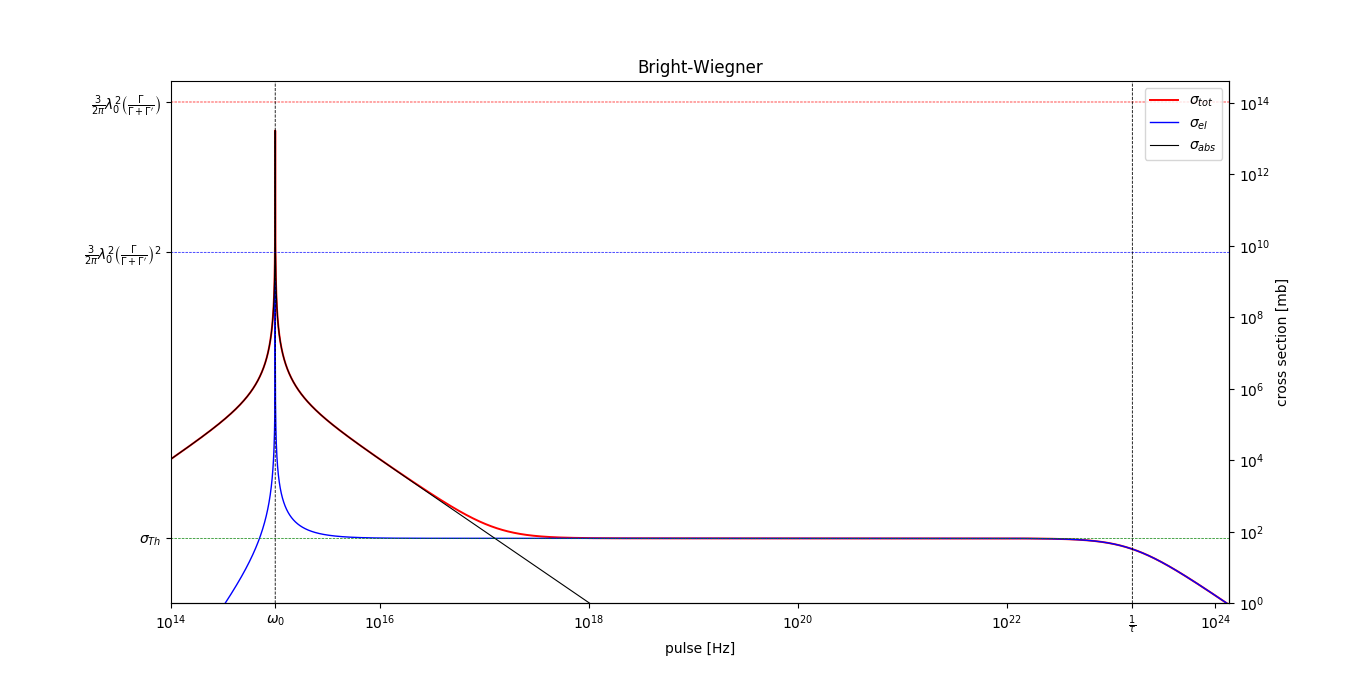
\includegraphics[width=1.1\textwidth]{immagini/b-w.png}
	\caption{Andamento delle sezioni d'urto della Bright-Wiegner}
	\label{fig:Andamento Bright-Wiegner}
\end{figure}
Nella figura si mostra come vanno le sezioni d'urto, è necessario notare che, per un rendering più fedele, sarebbero serviti più punti plottati (la funzione non ha raggiunto il massimo atteso). Per pigrizia è stato testato che arrivasse al massimo ma non è stata riportata l'immagine; insomma fidarsi o provare per credere.

%2.b.17
\subsection[]{Dimostrare che la sezione d’urto elastica per un’onda e.m. piana e monocromatica su un elettrone legato elasticamente in prossimità di una risonanza stretta (specificare il criterio) si può approssimare con una curva lorentziana
\[
	\sigma_{el} = \sigma_{Th} \frac{\omega_{0}^2 / 4}{ \left( \omega_0 - \omega \right)^2 + \frac{ \left( \Gamma' + \Gamma  \right)^2 }{4} }
\] 
}
La B-W si approssima con una lorenziana in un intorno (dell'ordine della larghezza $\Gamma + \Gamma'$) di $\omega_0$: $\omega \approx \omega_0$.\\
La risonanza è stretta se la larghezza a metà altezza è molto inferiore alla frequenza di risonanza: $\Gamma + \Gamma' \ll \omega_0$.
Passiamo alle approssimazioni allora:
\begin{align*}
	\sigma_{\text{el}} = \sigma_{\text{Th}}\frac{\omega ^{4}}{\left( \omega _0 - \omega\right)^2 \left( \omega_0 + \omega \right)^2 + \omega^2\left( \Gamma + \Gamma' \frac{\omega^2}{\omega_0^2} \right)^2} \approx \\
	\approx \sigma_{\text{Th}} \frac{\omega _0^4}{4 \omega _0^2 \left( \omega _0 - \omega  \right)^2 + \left( \Gamma + \Gamma' \right)^2 \omega _0^2  } \approx \\
	\approx \sigma_{\text{Th}}\frac{\omega_0^2/4}{\left( \omega - \omega_0 \right)^2 + \left(\frac{\Gamma + \Gamma'}{2}\right)^2 }
.\end{align*}

% 2.b.18
\subsection[]{Dimostrare che per un’onda e.m. piana e monocromatica su un elettrone legato elasticamente le sezioni d'urto al picco valgono:
\[
	\sigma_{el} = \frac{3 \lambda_{0}^2}{2 \pi} \left( \frac{\Gamma}{\Gamma + \Gamma'} \right)^2 \quad \quad \quad \quad \quad \quad \text{ }
\]
\[
	\sigma_{TOT} = \frac{3 \lambda_{0}^2}{2 \pi} \frac{\Gamma}{\Gamma + \Gamma'} \quad \quad \text{Con $\lambda_{0} = \frac{2 \pi c}{\omega_{0}}$}
\]
\[
	\sigma_{inel} = \frac{3 \lambda_{0}^2}{2 \pi} \frac{\Gamma \Gamma'}{\left( \Gamma + \Gamma' \right)^2 } \quad \quad \quad \quad \quad \quad \text{ } 
\]
}
Accettanto il fatto che tutte le tre sezioni d'urto hanno un massimo per $\omega = \omega_0$ basta prendere le sezioni d'urto e sbatterci dentro $\omega = \omega_0$.

%2.b.19
\subsection[]{Dimostrare che un elettrone (moto non relativistico) soggetto ad una forza elastica di richiamo, ad una forza di attrito viscoso ed alla forza di reazione radiativa, se viene lasciato libero di oscillare da una posizione iniziale perde energia con una 1 legge esponenziale in cui la costante tempo vale $\frac{1}{\Gamma' + \Gamma}$. Come si chiama questa costante tempo? Quale sarebbe la costante tempo con cui, invece, si smorza l'ampiezza delle oscillazioni?}
Riprendiamo l'equazione di moto dell'elettrone, tuttavia adesso togliamo la forzante dovuta all'onda incidente.
\[
	- \tau \dddot{\boldsymbol{x}} + \ddot{\boldsymbol{x}} + \Gamma' \dot{\boldsymbol{x}} + \omega_0^2 \boldsymbol{x} = 0 
.\]  
Adesso è necessario ricordare le relazioni tra i vari parametri in gioco:
\[
	\Gamma' \ll \omega_0 \ll \frac{1}{\tau}, \quad \quad \quad  
	\Gamma \ll \omega_0
.\] 
La prima è una questione puramente di grandezze fisicamente tipiche, la seconda deriva dalla prima $\left( \omega_0 \tau \ll 1 \right) $ e dal fatto che $\Gamma = \tau \omega_0^2 \ll 1 \cdot \omega_0$.\\
È quindi ragionevole cercare una soluzione oscillante e smorzante con smorzamento debole rispetto alla pulsazione:
\[
	\boldsymbol{x} = \boldsymbol{x}_0 e^{-i\left( \omega_0 - i \gamma/2 \right)t } = \boldsymbol{x}_0 e^{-i \omega_0t} e^{-\gamma t /2}, \quad \quad \quad 
	\gamma \ll \omega_0
.\]
Adesso la festa è nel sostituire questa soluzione nella equazione buttando via i termini trascurabili:
\[
	- \tau \left( -i\left( \omega_0 - i \gamma /2 \right)  \right)^3 + \left( -i\left( \omega_0 - i \gamma /2 \right) \right)^2 - \left( -i\left( \omega_0 - i \gamma /2 \right) \right) \Gamma' - \omega_0^2 = 0 
.\]
Sostituendo $\tau = \Gamma / \omega_0^2$:
\[
	-i \frac{\Gamma}{\omega_0^2}\left( \omega_0^3 - \frac{3}{2} i \gamma \omega_0^2 + \ldots \right) - \left( \omega_0^2 - i \gamma \omega_0 + \ldots \right) + 
	\left( -i \Gamma' \omega_0 - \frac{1}{2} \gamma \Gamma'  \right) + \omega_0^2 \approx 0 
.\] 
Sempre sulla base delle approssimazioni sopra è possibile notare che i termini reali sono trascurabili (raggruppare alcuni $\Gamma$ o $\Gamma'$ nei punti giusti per vederlo), ci si riduce alla forma:
\[
	-i \Gamma \omega_0 - \frac{3}{2} \Gamma \gamma - i \Gamma' \omega_0 + i \gamma \omega_0 - \frac{1}{2} \gamma \Gamma' \approx 0 \implies 
	- \Gamma \omega_0 - \Gamma' \omega_0 + \gamma \omega_0 \approx 0 
.\] 
Che ci porta alla conclusione:
\[
\gamma \approx \Gamma + \Gamma 
.\]
Quindi l'ampiezza delle oscilazioni è smorzata con una costante tempo data da:
\[
	\boldsymbol{x} = \ldots \cdot e^{- t /\tau_{\text{osc}}} \quad \quad \text{con} \quad \quad
\tau_{osc} = \frac{2}{\gamma} = \frac{2}{\Gamma + \Gamma'}
.\]
Se consideriamo invece l'andamento della energia è necessario tener conto del fatto che essa è quadratica nella velocità (cinetica) e nella posizione (potenziale): 
\[
E = E_0 e^{- \gamma t} \quad \implies \quad \tau_{\text{energia}} = \frac{1}{\gamma} = \frac{1}{\Gamma + \Gamma'}
.\]
In tutto questo macello il risultato importante è uno: la larghezza totale di uno stato risonante è il reciproco della sua vita media, risonanza stretta = particella longeva e viceversa.

% 2.b.20
\subsection[]{Calcolare la relazione tra parametro d'impatto (b) e angolo di scattering ($\theta$) nel caso di scattering di Rutherford (Coulombiano) e di scattering su sfera rigida.} 


% 2.b.21
\subsection[]{ Calcolare la minima distanza fra le due particelle in uno scattering Rutherford.}

\subsection[]{ Calcolare l'energia minima affinché un protone possa avere una interazione forte "toccando" un nucleo di ${}^{12}C$ o di ${}^{28} Si$.}

\subsection[]{ Discutere le differenze tra lo scattering di Rutherford (particelle $\alpha$ su nuclei) e lo scattering di elettroni su bersaglio puntiforme.}

\subsection[]{ Cercando i dati nelle apposite tabelle (reperibili sul web ) si indichino gli stati finali e si calcoli il Q-valore per i decadimenti delle seguenti specie instabili: ${}^8B, {}^{39}Ar, {}^{7}Be, {}^{64}Cu, {}^{76}Ge$. }

\subsection[]{ Cercando i dati nelle apposite tabelle (reperibili sul web) si trovino i Q-valori per le reazioni 
\begin{enumerate}
	\item $n + {}^{154}Gd \implies \gamma + {}^{155}Gd$ 
	\item $n + {}^{155}Gd \implies \gamma + {}^{156}Gd$
\end{enumerate}
}

\subsection[]{ Dimostrare che $\frac{d^3 p  }{2E}$ è un invariante relativistico effettuando esplicitamente la 2Etrasformazione di Lorentz (si consideri il boost lungo un asse, p. es. l'asse x)}

\subsection[]{ Dimostrare che $d^{4}p \delta\left( p^2-m^2 \right) \theta\left( p_0 \right) = \frac{d^3 p }{2E}$  e sfruttare questo risultato per semplificare la scrittura dell’elemento infinitesimo dello spazio dei 4-impulsi di N particelle emergenti dopo la collisione di due particelle (oppure dopo il decadimento di una particella).}

\subsection[]{ Dimostrare che nel centro di massa l’elemento infinitesimo dello spazio dei 4-impulsi, nel caso di 2 sole particelle nello stato finale, si scrive come $\frac{|\boldsymbol{p_{cm}}}{4\sqrt{s}} d\Omega_{cm}.$}

\subsection[]{ Nel caso di 3 particelle nello stato finale di una reazione, dimostrare che fra il quadrato della massa invariante di due di esse e l'energia della terza (nel centro di massa) sussite una relazione lineare.}

\subsection[]{ Come si trasforma una funzione di distribuzione del 3-impulso $f\left( \boldsymbol{p} \right)d^3 \boldsymbol{p}$ di una
particella per una trasformazione di Lorentz?}

\subsection[]{ Come si trasforma una funzione di distribuzione nello spazio delle fasi 
\[
	f\left(\boldsymbol{p},\boldsymbol{r}\right)d^3 \boldsymbol{p} \ d^3 \boldsymbol{r} 
\]
di una particella per una trasformazione di Lorentz?}

\subsection[]{ Dimostrare che se la probabilità di decadimento di una particella per unità di tempo non dipende dal tempo, la probabilità di trovare la particella non decaduta al tempo t segue una legge esponenziale.}

\subsection[]{ Dire quali fra le seguenti particelle sono soggette ad interazioni forti: $ p, \overline{p} $, $\pi^{+}, \pi^{-}, \mu^{+}, \mu^{-}, e^{+}$, $e^{-}$, $\alpha,$ Nucleo di Azoto, $\nu, \overline{\nu}$ }

\subsection[]{ Pioni neutri, di energia E nel sistema del laboratorio, decadono in due fotoni. La distribuzione è isotropa ne centro di massa. Si calcoli la distribuzione dell’energia di uno dei due fotoni nel laboratorio e gli angoli, rispetto alla direzione di volo del pione, dei due fotoni nel sistema del laboratorio in funzione dell’angolo nel sistema del centro di massa.}

\subsection[]{ Calcolare la funzione di distribuzione in energia ed in angolo nel sistema del laboratorio di un fascio di neutrini o di muoni prodotto nel decadimento di pioni carichi di energia 14 GeV.}

\subsection[]{ Qual e' l'andamento delle masse nucleari a parità di A in funzione di Z?}

\subsection[]{ Dimostrare che in un tipico decadimento $\alpha$, la particella $\alpha$ emerge con circa il 98\% dell'energia disponibile.}

\subsection[]{ Dimostrare che in un decadimento $\beta$ la somma delle energie dell'elettrone e dell'antineutrino emessi é praticamente uguale al Q-valore della reazione.}
